% !Mode:: "TeX:UTF-8"
%!TEX program  = xelatex

\documentclass{cumcmthesis}
	%\documentclass[withoutpreface,bwprint]{cumcmthesis} %去掉封面与编号页
	
	\usepackage{url}
	\usepackage{amssymb}
	\begin{document}
	
	\begin{abstract}
	
	\keywords{决策模型\ \ }
	\end{abstract}
	
	%目录
	\tableofcontents
	
	\section{问题重述}
	\subsection{问题背景}
	一个智能加工系统由8台计算机数控机床 (Computer Number Controller, CNC)、1辆轨道式自动导引车 (Rail Guide Vehicle, RGV)、1条RGV直线轨道、1条上料传送带、1条下料传送带等附属设备组成。RGV是一种无人驾驶、能在固定轨道上自由运行的智能车。它根据指令能自动控制移动方向和距离,并自带一个机械手臂、两只机械手爪和物料清洗槽,能够完成上下料及清洗物料等作业任务。\cite{Saiti}通常来说,一个工件成品的完成需要若干步,鉴于RGV小车在同一时间只能处理同一种任务,而同时最多可以有8台数控机床在运行,因此对RGV小车进行正确的调度将显著地提高该智能加工系统的加工效率。在本文中,我们将运用不同模型讨论在不同情形下,如何调度小车能够使该系统达到最高效的工作状态。
	
	\subsection{问题提出}
	根据以上的背景,我们在本文中需要针对下面的三种具体情况:
	
	\begin{itemize}
		\item 一道工序的物料加工作业情况,每台CNC安装同样的刀具,物料可以在任一台CNC上加工完成;
		\item 两道工序的物料加工作业情况,每个物料的第一和第二道工序分别由两台不同的CNC依次加工完成;
		\item CNC在加工过程中可能发生故障(据统计:故障的发生概率约为1\%)的情况,每次故障排除(人工处理,未完成的物料报废)时间介于10~20分钟之间,故障排除后即刻加入作业序列。要求分别考虑一道工序和两道工序的物料加工作业情况。
	\end{itemize}
	
	完成两项任务:\newline
	任务1:对一般问题进行研究,给出RGV动态调度模型和相应的求解算法;\newline
	任务2:利用已给出的系统作业参数的3组数据分别检验模型的实用性和算法的有效性,给出RGV的调度策略和系统的作业效率。
	
	\section{模型的假设}
	基于赛题中给出的一些条件和生活常识,我们在本文中提出如下假设。此后在用到这些假设时,我们将不再另作声明。
	\begin{itemize}
	\item RGV小车需要对某台数控机床上下料作业时,数控机床对应的传送带上一定有一个预备好的原料工件;
	\item RGV小车不能同时进行两项或以上的工作 (包括移动);
	\item 
	\end{itemize}
	
	
	\section{符号说明}
	\begin{table}[!htbp]
		\centering
		\begin{tabular}{cc}
		\toprule[1.5pt]
		符号 & 意义\\
		\midrule[1pt]
		alg     & 调度算法/调度方案 \\
		$n_t$ & 在$t$时间内加工完的工件数  \\
		$T_0$ & 情况一CNC由原料加工为成品的时间 \\
		$T_1$ & 情况二CNC由原料加工为半成品的时间 \\
		$T_2$ & 情况二CNC由半成品加工为成品的时间 \\
		$T_{move k}$ & RGV移动$k$步所花的时间($k\in{1, 2, 3}$) \\
		$T_{wash}$ & RGV清洗所花的时间 \\
		$T_{load odd}$ & RGV为奇数号CNC上下料所花的时间 \\
		$T_{load even}$ & RGV为偶数号CNC上下料所花的时间 \\
		20 & 640.2 \\
		\bottomrule[1.5pt]
		\end{tabular}
		\caption{文中用到的符号和含义}\label{fuHaoShuoMing}
	\end{table}
	
	\section{问题分析}
	我们将针对本问题给出的三种情况分别予以分析,并提出可能的优化算法。
	\subsection{情况一、二分析}
	在情况一中,一个工件只需经过一步加工就可以成为成品,然后经过RGV小车清洗后放入下料传送带送出该系统。此时,一个工件从原料到成品需要RGV小车的如下操作:
	\begin{enumerate}
		\item 移动步骤:RGV小车从原来的位置运行到CNC的位置;
		\item 第一次上下料步骤:小车将上料传送带上的原料取下,将CNC中的成品置换为原料,若CNC原来处于空置状态,则只将原料放入CNC中;
		\item 等待:等待CNC加工完成,此时小车可以进行其他任务;
		\item 第二次上下料步骤:小车再次运行到CNC的位置,将CNC中的成品置换为原料,此时小车不能为已装载成品的状态;
		\item 清洗步骤:小车清洗成品,并将成品置入下料传送带上。
	\end{enumerate}
	而在情况二中,一个工件需要两步加工才能制成成品,因此工件由原料到成品需要多一次上下料步骤,即在第一轮加工完成后,将加工完成的工件放入第二步工序的CNC中加工。其他的步骤均是相同的。\newline
	显然,因为不存在任何随机因素,因此所有小车调度方案的数量是有限的,故情况一、二的全局最优解是一定存在并且确定的,意即:
	\[\exists\textrm{alg}\ \textrm{s.t.}\ n_{t, \textrm{alg}}=\textrm{Max}[n_t]\]
	所以我们需要找到该最优的调度方案或接近最优的调度方案。\newline
	要得到最优的调度方案,可能可以使用的算法有:穷举法、模拟退火算法、决策树算法、遗传算法、神经网络等。其中,穷举法和模拟退火算法的时间复杂度过高,超过了我们所拥有的算力极限,故我们不考虑用此两种方法。同样是基于统计的算法,遗传算法在该题中表现出比模拟算法更优的时间性能,因此遗传算法将成为我们探寻最优解的一种尝试。
	
	\subsection{情况三分析}
	对于情况三,由于加入了随机因素(CNC发生故障),因此不存在固定的全局最优解。在此情况下,调度过程转化成了小车的决策过程。空闲的小车需要灵活地根据当前加工系统的状态来决定下一步将要进行的步骤。在该情况下,遗传算法仍然可以使用,但是由原来的提供静态方案转变为即时演算出动态决策。
	
	\section{模拟环境}
	为了能够实际测试调度算法产生的指令序列在RGV智能加工系统中的表现,我们基于题目中给出的文档与数据,设计了一个简易的智能加工系统模拟器。每当RGV小车处于空闲状态时,模拟器会将当前智能加工系统各部分的状态以及当前的时刻作为参数传递给调度算法,调度算法会以此作为输入进行计算,并且输出当前小车需要执行的指令。
	
	模拟器使用python设计,主要由4个模块组成。它们分别是world.py,rgv.py,cnc.py以及cargo.py。
	
	world.py是模拟器的核心部分。在world.py中包含模拟器的主对象World,构造该对象时需要传入工作时间或者加工工件总数,以及调度器作为参数。对象构造完成后,调用对象的simulate()方法就可以开始模拟。模拟结束后,可以调用result()和final()方法获得加工的工件个数/加工的总时间长,以及每一个工件上料和下料的时间日志记录。
	
	rgv.py包含了RGV对象,其中定义了RGV可以接受的指令和它们的编码,它们在模拟器中的对应关系如下表所示。
	
	\begin{table}[!htbp]
		\centering
		\begin{tabular}{c|c}
			\toprule[1.5pt]
			编码 & 指令 \\
			\midrule[1pt]
			0 & 空闲 \\
			1 & 向左移动一格\\
			2 & 向右移动一格\\
			3 & 向左移动两格\\
			4 & 向右移动两格\\
			5 & 向左移动三格\\
			6 & 向右移动三格\\
			7 & 向\#1,\#3,\#5,\#7号CNC上下料\\
			8 & 向\#2,\#4,\#6,\#8号CNC上下料\\
			9 & 清洗工件\\
			\bottomrule[1.5pt]
		\end{tabular}
		\caption{RGV的指令和编码}\label{rgv指令和编码}
	\end{table}
	
	RGV对象可以通过inst()方法来接受指令。调用这个方法时需要传入一个有效指令的编码,同时根据指令的种类传入一个可选参数,类型为代表工件的Cargo类。关于Cargo类的信息会在下文描述。调用该方法后会设置RGV内部的一些属性,包括对象内部的计时器。
	
	同时,RGV对象也拥有update()方法,调用这个方法时,如果RGV正在执行空闲之外的指令,那么程序会将RGV内部的计时器减少1秒。接着,程序将会检查RGV内部的计时器是否已经达到零。如果计时器已经达到零,那么表明当前指令已经执行完成,那么RGV对象会根据指令的不同执行一些动作,比如修改CNC机床内部的工件对象或者修改自身内部的工件状态。
	
	cnc.py包含了CNC对象。CNC对象的可能状态如下表所示:
	
	\begin{table}[!htbp]
		\centering
		\begin{tabular}{c|c}
			\toprule[1.5pt]
			编码 & 指令 \\
			\midrule[1.5pt]
			0 & 空闲 \\
			1 & 加工中\\
			2 & 加工完成\\
			3 & 故障\\
			\bottomrule[1.5pt]
		\end{tabular}
		\caption{CNC对象的可能状态}
	\end{table}
	
	与RGV对象类似,CNC对象也拥有inst()方法与update()方法。它们的功能也与RGV对象中的对应方法类似。
	
	由于智能加工系统的要求,CNC对象拥有不同模式。可能的模式如下表所示:
	\begin{table}[!htbp]
		\centering
		\begin{tabular}{c|c}
			\toprule[1.5pt]
			编码 & 状态 \\
			\midrule[1.5pt]
			0 & 一阶段加工 \\
			1 & 二阶段加工,第一阶段\\
			2 & 二阶段加工,第二阶段\\
			\bottomrule[1.5pt]
		\end{tabular}
		\caption{CNC对象的可能模式}
	\end{table}
	
	cargo.py内部包含Cargo对象。Cargo对象的状态如下表所示:
	\begin{table}[!htbp]
		\centering
		\begin{tabular}{c|c}
			\toprule[1.5pt]
			编码 & 状态 \\
			\midrule[1.5pt]
			0 & 未加工 \\
			1 & 半加工\\
			2 & 加工完成,未清洗\\
			3 & 加工完成,已清洗\\
			\bottomrule[1.5pt]
		\end{tabular}
		\caption{Cargo(工件)对象的可能状态}
	\end{table}
	Cargo(工件)对象的状态可以用RGV对象和CNC对象中的相应指令来修改。同时,保存工件的状态也使得模拟器能够检测出输入的指令序列中的错误,防止不能出现的情况发生。
	
	为了调试方便,我们为模拟器添加了输出函数info()。输出示例如下:
	
	\begin{lstlisting}
		supply cargo 2
		Clock: 3931
		RGV:        CNC 1:      CNC 2:      CNC 3:      CNC 4:      CNC 5:      CNC 6:      CNC 7:      CNC 8:
		idle        processed   processed   idle        idle        processed   processing  idle        idle
		8, ready    4, ready    5, ready                            7, ready    9, raw
		current cargo: 9
	\end{lstlisting}
	
	模拟结束后,模拟器会将数据写入对应的文件中。
	
	\section{标准调度模型}
	为了能够定量的评价后续模型的优劣,我们按照题意设计了一个标准调度模型,来与之后的模型对比。标准调度模型是一种确定性模型,由人来确定小车调度中应当依次完成工作的优先级,然后小车就依照确定的优先级处理CNC发送的请求。

	\subsection{情况一的标准调度模型}
	对于情况一,标准调度模型基于以下几条原则:
	\begin{itemize}
		\item 小车会优先执行完当前的指令队列,然后再接收CNC的服务请求;
		\item 在所有CNC都工作时,若小车的执行队列为空,则小车处于空闲状态;
		\item 若只有一台CNC处于可服务状态,小车将会为这台CNC提供服务;
		\item 若有多台CNC处于可服务状态,小车将会优先服务近的、奇数号的CNC;
		\item 在完成一次上下料作业后,若需要清洗,小车会立即进行清洗。
	\end{itemize}
	在这个情况下,小车的调度成为了一个确定问题。在每次小车处于空闲状态时,它可能会接收多个CNC的服务请求,但是它将要执行的指令其实已经确定了。我们可以认为,小车会将CNC的优先级按照距离和奇偶性排序。在它接收了多个CNC的服务请求以后,将按照图 \ref{StandardModelCondition1} 所示的流程依次判断服务对象,然后将整个服务流程所需的步骤编入其指令队列。例如,若小车处于位置1,而编号为3,4,5,7的CNC需要服务,那么小车会按照1,2,……,7,8的顺序询问CNC是否需要服务。最终,小车将对编号为3的机器提供服务。
	\begin{figure}
		\centering
		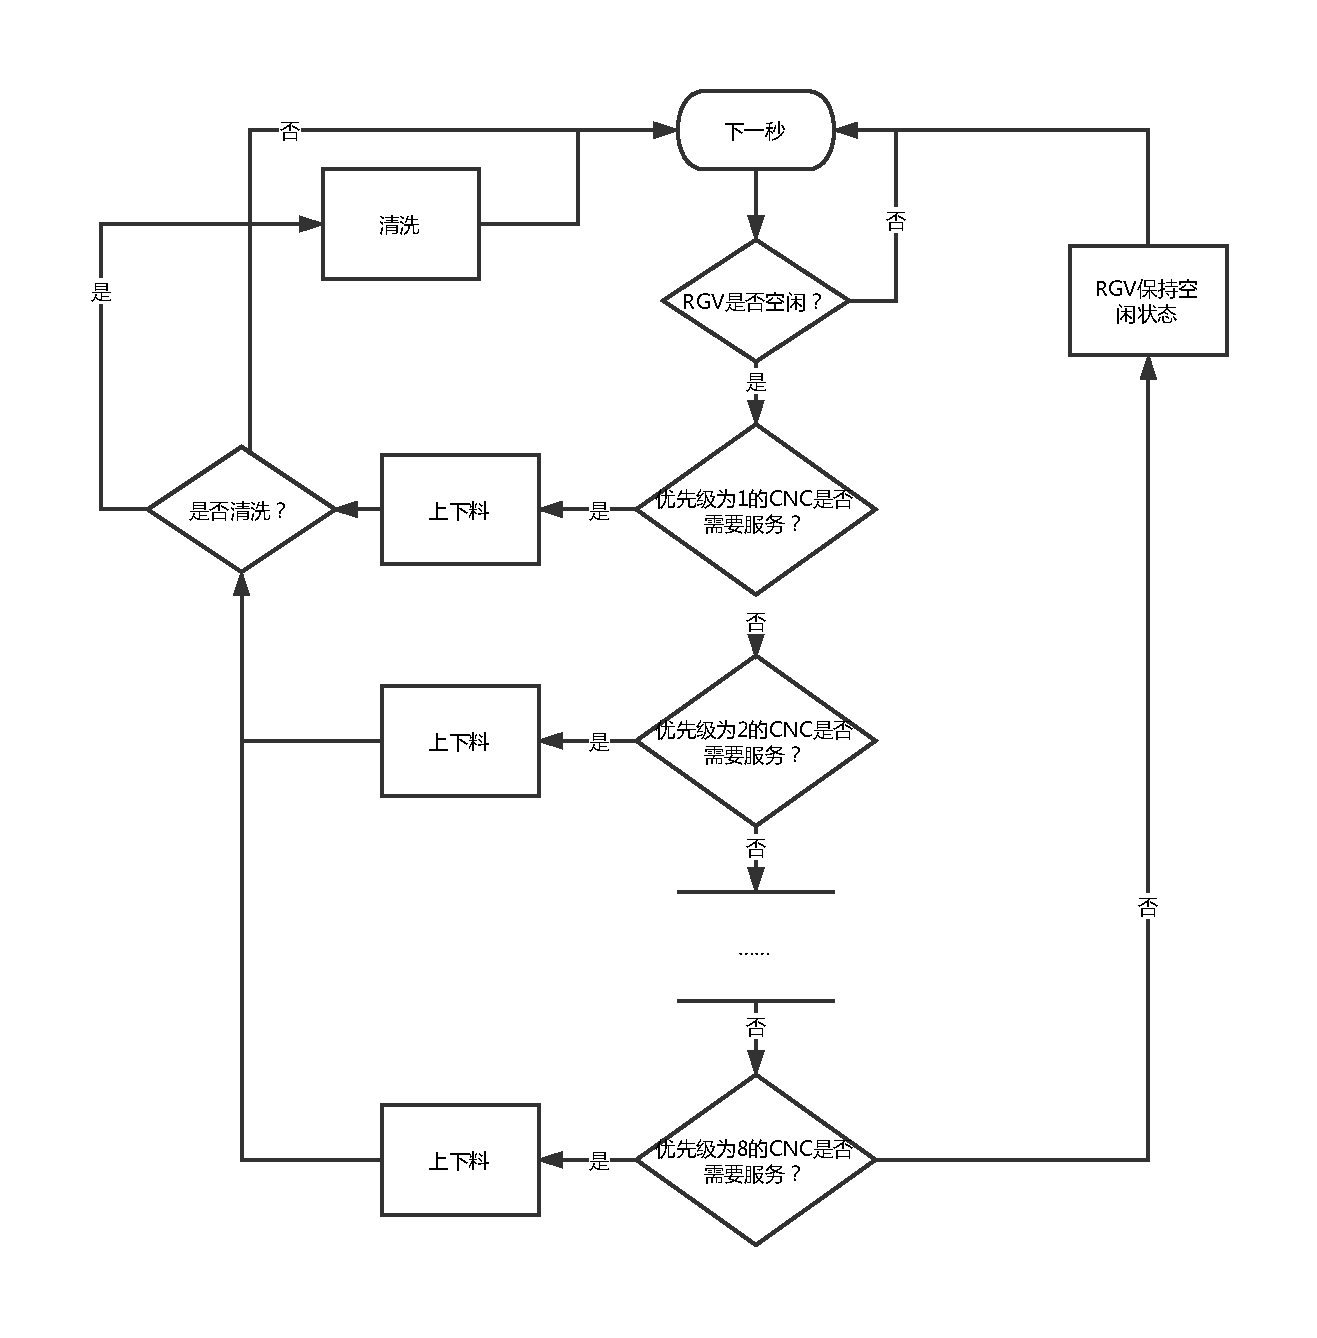
\includegraphics[width=.7\linewidth]{simple_model_1.pdf}
		\caption{标准模型(情况一)的运行流程}\label{StandardModelCondition1}
	\end{figure}
	在有机器出现故障的情况下,该标准模型仍能正常工作。

	\subsection{情况二的标准调度模型}
	对于情况二,一个工件从原料到成品需要两个工序,依次经过两台CNC。因此,我们对情况一的原则稍加改动,引入情况二标准模型的几条原则:
	\begin{itemize}
		\item 小车会优先执行完当前的指令队列,然后再接收CNC的服务请求;
		\item 在所有CNC都工作时,若小车的执行队列为空,则小车处于空闲状态;
		\item 若小车当前只能为一台CNC提供服务,则小车将会为这台CNC提供服务;
		\item 若小车当前能为多台CNC提供服务,则小车会按照先服务第一工序CNC,再服务第二工序CNC;先近后远;先奇后偶的顺序依次对要服务的CNC进行排序,然后服务第一顺序的CNC;
		\item 在完成一次上下料作业后,若需要清洗,小车会立即进行清洗。
	\end{itemize}
	同样地,在情况二下小车调度也是一个确定问题,流程如图 所示。

	\section{情况一的解}
	\subsection{标准调度模型}
	使用标准调度模型可以快速地得到一个基本令人满意的解。鉴于标准调度模型的时间复杂度为\(O(n)\),标准调度模型测试程序运行需要的时间非常短,约在 秒以内。而此模型的结果为:在8小时内共有 个成品被送上了下料传送带,如图 所示。
	
	\subsection{遗传算法}


	\subsection{最优解}
	经过观察和验证,我们认为我们得到了情况一下一种特殊情况的最优解。当该加工系统的各项时间满足
	\[T_0 \geq 3T_{move 1}+T_{move 3}+8T_{wash}+3T_{load odd}+4T_{load even}\]
	时,在标准模型的基础上增加一条原则:
	\begin{itemize}
		\item 当小车没有需要服务的对象而自身空闲时,小车将前往最快要完成的CNC旁等候。
	\end{itemize}
	该情况下,8小时内加工完成的工件数达到所有情况下能达到的最大值。接下来我们对其进行证明:
	\begin{lemma}
		在一定时间$t$内($t$足够大),若所有CNC的总等待时间最小,则加工完成的工件数达到最大。
	\end{lemma}
	\begin{proof}
		设在$t$内,所有CNC的最小总等待时间为$T$,此时加工完成的工件数为$n_t$,则有:
		$$8t-n_tT_0>T\geq \textrm{Max}[0, 8t-n_tT_0-8T_0]$$
		因此若$T'>8t-n_tT_0$,则显然此时$n_t'<n_t$。\newline
		若$8t-n_tT_0>T'>T$,而$n_t'>n_t$,则有$\hfill\blacksquare$
	\end{proof}
	\begin{theorem}
		小车空闲时,若有多台CNC请求服务,小车应当先应对耗时最短的服务请求。
	\end{theorem}
	\begin{proof}
		设有$k$台CNC向小车发送了服务请求,其服务需要的时间分别为$t_1<t_2<...<t_k$,则小车先为第$i$台CNC服务所产生的总等待时间为$k\cdot t_i$,取$t_1$可使总等待时间最小化,之后由引理1即可得证。$\hfill\blacksquare$
	\end{proof}
	由该定理我们验证了小车对不同CNC进行排序服务原则的合理性。
	\begin{theorem}
		小车空闲时,若没有CNC请求服务,小车应当前往最快要完成的CNC旁等候。
	\end{theorem}
	\begin{proof}
		对任意的CNC来说,若小车完成了一次上下料任务,则小车为其他CNC完成上下料,再返回当前CNC的位置所需的时间最大值为
		\[T_{needMax}=3T_{move 1}+T_{move 3}+8T_{wash}+3T_{load odd}+4T_{load even}\]
		而下一次该CNC需要上下料服务的时间为$T_0>T_{needMax}$
		因此在RGV完成其他上下料任务后,其应当返回该CNC处准备对该CNC进行上下料任务。此时,该CNC即为最快要完成的CNC。$\hfill\blacksquare$
	\end{proof}
	对于其他原则,我们认为其十分显然,就不再给出额外的证明。由此,我们可以获知该调度模型即为最优的调度模型。特殊地,对于情况一,该调度模型可以简化为一个周期性调度方案:
	\begin{center}
	\fangsong
	RGV为CNC1上下料(含清洗)$\Rightarrow$RGV为CNC2上下料(含清洗)$\Rightarrow$...\newline$\Rightarrow$RGV为CNC8上下料(含清洗)$\Rightarrow$RGV回到位置1\newline$\Rightarrow$等待CNC1完成$\Rightarrow$RGV为CNC1上下料(含清洗)$\Rightarrow$...
	\end{center}
	该最优算法可以使加工系统在8小时内完成383(数据组1)和392(数据组3)个成品,远远超过了标准模型和遗传算法模型的效率。而数据组2虽然在此情况下并非最优解,但是也在8小时内完成了360个成品,其效率仍然超过了标准模型和遗传算法模型。

	\section{情况二的解}
	对于情况二,CNC的分配在模型中也是十分重要的一个因素。我们认为CNC的分配应当遵从平均原则,即通过给加工时间长的CNC赋予更短的平均服务时间和更多的数量来使CNC与RGV的工作更为协调。因此,对于给出的三组数据:
	
	\subsection{标准调度模型}
	同样地,应用在情况二中,标准调度模型依然可以得到一个可以接受的解。用标准调度模型运行情况二的系统分别可以在8小时内完成 个成品。

	\subsection{遗传算法}
	\subsection{遗传算法的并行化}
	遗传算法需要计算每一代个体的适应度。如果将$v_{ch}$作为染色体向量,$v_{ch}^{(i)}$作为第$i$个个体的染色体,那么适应度的计算可以抽象成一个函数$h(v_{ch}^{(i)})=v_{ch}^{(i)}\rightarrow\mathbf{R}$,对于整代个体来说就是计算$h(v_{ch})=[h(v_{vh}^{(1)}),h(v_{vh}^{(2)}),...,h(v_{vh}^{(k)})]^T$。这一部分计算需要使用模拟世界来得出生产的工件数量,需要消耗较长的时间,因此将这部分内容并行化,加速算法的计算。
	
	实现上使用了python的mutiprocessing包,使用了其中的进程池Pool的map()方法来完成遗传算法的并行化。这样,python解释器会创建多个进程,并行地计算个体的适应度。代码如下:
	\begin{lstlisting}[language=python]
	import multiprocessing
	
	cores = multiprocessing.cpu_count()
	pool = multiprocessing.Pool(processes=cores)
	
	fitness_values = pool.map(
		Functor,
		chromosome_pairs
	)
	
	pool.close()
	pool.join()
	\end{lstlisting}
	
	\subsection{不同的编码方式}
	
	值得注意的是,RGV在智能加工系统中收到的指令序列常常具有周期性。然而简单的将目标CNC的编号作为个体的染色体编码不能体现这种周期性的特征。因此,我们设计了另一种编码,以体现这种周期性的特征。
	
	每个个体的染色体为长度为p的向量,向量p的元素是等长(q)的序列,序列中代表某一个周期内RGV小车的目标CNC的序列。例如$$v_{ch}^{(m)} = (\{1,2,3,4,5,6,7,8\},\{8,7,6,5,4,3,2,1\})$$就是一个长度为2的编码。染色体的重组是将序列作为整体进行重组,但是每一个序列内部的顺序没有变化。而染色体的突变就是随机选择编码中的某个序列进行重排shuffle(),使序列内部的顺序发生变化。
	
	基于这种编码方式,我们重新实现了遗传算法,并且尝试对单阶段加工与二阶段加工进行优化。通过调整编码的长度和序列的长度,我们可以得到相对原有遗传算法较好的结果。

	\section{情况三的解}
	\subsection{情况3-1}
	情况3-1用情况1的最优解仍然能够实现。因为机器故障可以视为强制增加的等待时间,因此最优解的证明对情况3-1仍然有效。由此可以得到3-1的解,在此不再赘述了。
	\subsection{情况3-2}
	对有故障的双工序作业,要通过遗传算法来解决调度问题是十分困难的。我们的遗传算法使用的是确定性序列,而由于故障是随机因素,故障的存在会使得遗传算法的训练受到很大程度的影响,导致优秀的基因被筛去或
	
	%参考文献
	\begin{thebibliography}{9}
		\bibitem{Saiti} 2018年全国大学生数学建模竞赛B题,cumcm.cnki.net,2018.9.13
	\end{thebibliography}
	
	\newpage
	%附录
	\appendix
	\section{排队算法--matlab 源程序}
	\begin{lstlisting}[language=matlab]
	kk=2;[mdd,ndd]=size(dd);
	while ~isempty(V)
	[tmpd,j]=min(W(i,V));tmpj=V(j);
	for k=2:ndd
	[tmp1,jj]=min(dd(1,k)+W(dd(2,k),V));
	tmp2=V(jj);tt(k-1,:)=[tmp1,tmp2,jj];
	end
	tmp=[tmpd,tmpj,j;tt];[tmp3,tmp4]=min(tmp(:,1));
	if tmp3==tmpd, ss(1:2,kk)=[i;tmp(tmp4,2)];
	else,tmp5=find(ss(:,tmp4)~=0);tmp6=length(tmp5);
	if dd(2,tmp4)==ss(tmp6,tmp4)
	ss(1:tmp6+1,kk)=[ss(tmp5,tmp4);tmp(tmp4,2)];
	else, ss(1:3,kk)=[i;dd(2,tmp4);tmp(tmp4,2)];
	end;end
	dd=[dd,[tmp3;tmp(tmp4,2)]];V(tmp(tmp4,3))=[];
	[mdd,ndd]=size(dd);kk=kk+1;
	end; S=ss; D=dd(1,:);
	 \end{lstlisting}
	\begin{lstlisting}[language=c]
	kk=2;
	[mdd,ndd]=size(dd);
	while ~isempty(V)
		[tmpd,j]=min(W(i,V));tmpj=V(j);
	for k=2:ndd
		[tmp1,jj]=min(dd(1,k)+W(dd(2,k),V));
		tmp2=V(jj);tt(k-1,:)=[tmp1,tmp2,jj];
	end
		tmp=[tmpd,tmpj,j;tt];[tmp3,tmp4]=min(tmp(:,1));
	if tmp3==tmpd, ss(1:2,kk)=[i;tmp(tmp4,2)];
	else,tmp5=find(ss(:,tmp4)~=0);tmp6=length(tmp5);
	if dd(2,tmp4)==ss(tmp6,tmp4)
		ss(1:tmp6+1,kk)=[ss(tmp5,tmp4);tmp(tmp4,2)];
	else, ss(1:3,kk)=[i;dd(2,tmp4);tmp(tmp4,2)];
	end;
	end
		dd=[dd,[tmp3;tmp(tmp4,2)]];V(tmp(tmp4,3))=[];
		[mdd,ndd]=size(dd);
		kk=kk+1;
	end;
	S=ss;
	D=dd(1,:);
	 \end{lstlisting}
	
	
	\end{document} 